\documentclass[12pt, twocolumn]{article}

% 引入相关的包
\usepackage{amsmath, listings, fontspec, geometry, graphicx, ctex, color, subfigure, amsfonts, amssymb}
\usepackage{multirow}
\usepackage[table,xcdraw]{xcolor}
\usepackage[ruled]{algorithm2e}
\usepackage[hidelinks]{hyperref}

		\usepackage{graphicx}
		\usepackage[most]{tcolorbox}
\hypersetup{
	colorlinks=true,
	linkcolor=red,
	citecolor=red,
}
\usepackage{booktabs}
\usepackage{multirow}
\usepackage{picins}

% 设定页面的尺寸和比例
\geometry{left = 1.5cm, right = 1.5cm, top = 1.5cm, bottom = 1.5cm}

% 设定两栏之间的间距
\setlength\columnsep{1cm}

% 设定字体,为代码的插入作准备
\newfontfamily\ubuntu{Ubuntu Mono}
\newfontfamily\consolas{Consolas}

% 头部信息
\title{\normf{编程:观测值逐次更新的扩展卡尔曼滤波器}}
\author{\normf 姓名:陈烁龙\;\;\;学号:2023202140019\;\;\;学院:测绘学院}
\date{\normf{\today}}

% 代码块的风格设定
\lstset{
	language=C++,
	basicstyle=\small\ubuntu,
	keywordstyle=\textbf,
	stringstyle=\itshape,
	commentstyle=\itshape,
	numberstyle=\scriptsize\ubuntu,
	showstringspaces=false,
	numbers=left,
	numbersep=8pt,
	tabsize=2,
	frame=single,
	framerule=1pt,
	columns=fullflexible,
	breaklines,
	frame=shadowbox, 
	backgroundcolor=\color[rgb]{0.97,0.97,0.97}
}

% 字体族的定义
% \fangsong \songti \heiti \kaishu
\newcommand\normf{\fangsong}
\newcommand\boldf{\heiti}
\newcommand\keywords[1]{\boldf{关键词:} \normf #1}

\newcommand\liehat[1]{\left[ #1 \right]_\times}
\newcommand\lievee[1]{\left[ #1 \right]^\vee}
\newcommand\liehatvee[1]{\left[ #1 \right]^\vee_\times}

\newcommand\mlcomment[1]{\iffalse #1 \fi}
%\newcommand\mlcomment[1]{ #1 }

\newcounter{problemname}
\newenvironment{problem}{\stepcounter{problemname}\par\noindent\normf\textbf{\textcolor[rgb]{1,0,0}{题目\arabic{problemname}.} }}{\leavevmode\\\par}
\newenvironment{solution}{\par\noindent\normf\textbf{解答: }}{\leavevmode\\\par}
\newenvironment{note}{\par\noindent\normf\textbf{题目\arabic{problemname}的注记: }}{\leavevmode\\\par}


\begin{document}
	\begin{titlepage}
	    \centering
	    \includegraphics[width=0.4\textwidth]{whu_red.png}\par\vspace{1cm}
	    \vspace{4cm}
	    {\huge\kaishu “机器视觉”讨论二\par 基于连续时间的多卷帘快门相机的无靶标\par 时空标定方法 \par}
	    \vspace{3cm}
	    {\Large\kaishu 
	    \begin{center}\begin{tabular}{l}
	    姓名:陈烁龙\\
	    学号:\bfseries 2023202140019\\
	    学院:测绘学院
	    \end{tabular}\end{center}
	     \par}
	    
	
	    \vfill
	
	% Bottom of the page
	    {\large\kaishu\bfseries \today\par}
	\end{titlepage}
		% 换页
 		\thispagestyle{empty}
		\clearpage
		
		% 插入目录、图、表并换页
		\pagenumbering{roman}
		\tableofcontents
		\newpage
		\listoffigures
		% 罗马字母形式的页码
		
		\clearpage
		% 从该页开始计数
		\setcounter{page}{1}
		% 阿拉伯数字形式的页码
		\pagenumbering{arabic}
	
	\section{\normf{研究背景与现状}}
	\normf
	\subsection{\normf{多相机融合}}
	多传感器融合是一种将多个传感器的数据进行融合的技术. 传感器融合技术可以提高传感器的精度和可靠性,同时也可以减少传感器的误差. 传感器融合技术在军事、航空、航天、工业、医疗等领域都有广泛的应用.
	
	在多传感器融合技术中,融合的数据可以是来自不同传感器的数据,也可以是来自同一传感器的多个数据. 传感器融合技术的研究主要包括传感器数据融合算法、传感器数据融合模型、传感器数据融合系统等方面.
	
	在自动驾驶领域,常用的传感器包括激光雷达、摄像头、毫米波雷达、GPS、惯性测量单元(IMU)等. 这些传感器可以提供车辆周围的环境信息,如障碍物、道路标志、车道线、地图等,以帮助自动驾驶系统做出决策和规划行驶路径. 其中应用得最为广泛的多传感器融合是多相机融合,其优势有:
	\begin{enumerate}
		\item 视野范围: 集成多个摄像头意味着可以获得更多视野,从而在存在视觉障碍的场景(例如行人或车辆交通繁忙的空间以及狭窄的空间)中具有更高的鲁棒性。
		在这种情况下,一旦摄像头被遮挡,单视觉系统就会失败,但多视觉系统则不会。
		
		\item 深度确定能力: 单目视觉系统没有尺度确定的能力,因此特征的深度是未知的。 虽然借助 IMU 可以解决这个问题,但需要复杂的算法。 通过集成具有精确时空参数的多个相机,可以通过三角化轻松确定特征深度和尺度。 这也可以很大程度上克服尺度漂移。
		
		\item 更高的精度: 集成多个 IMU 和相机意味着可以获得更多的测量结果,从而可以在估计器中很好地抑制观测噪声,从而提高精度。
		
		\item 更好的容错能力: 多个传感器可以带来更好的容错能力。
	\end{enumerate}
	\subsection{\normf{卷帘快门相机}}
	卷帘快门相机(rolling shutter camera, RS camera)是一种使用卷帘快门来控制曝光时间的相机。与全局曝光相机(global shutter camera, GS camera)同时曝光整幅影像不同,卷帘快门相机采用行曝光的形式生成图像,每行的时间都不同,但是间隔相同。与全局曝光相机相比,卷帘快门相机的主要优点是可以拍摄高速运动的物体,因为它可以在快门关闭之前暴露一部分图像,从而捕捉到物体的运动轨迹。然而,卷帘快门相机的缺点是在拍摄快速移动的物体时,可能会出现图像扭曲或失真的情况,也即RS效应,如图\ref{fig:卷帘快门畸变效应}、图\ref{fig:卷帘快门拍摄飞机螺旋桨产生的畸变效应}所示。
	
	\begin{figure}[h]
		\centering
		\includegraphics[width=\linewidth]{img/rs_camera_distort.png}
		\caption{\normf 卷帘快门畸变效应}
		\label{fig:卷帘快门畸变效应}
	\end{figure}
	
	\begin{figure}[h]
		\centering
		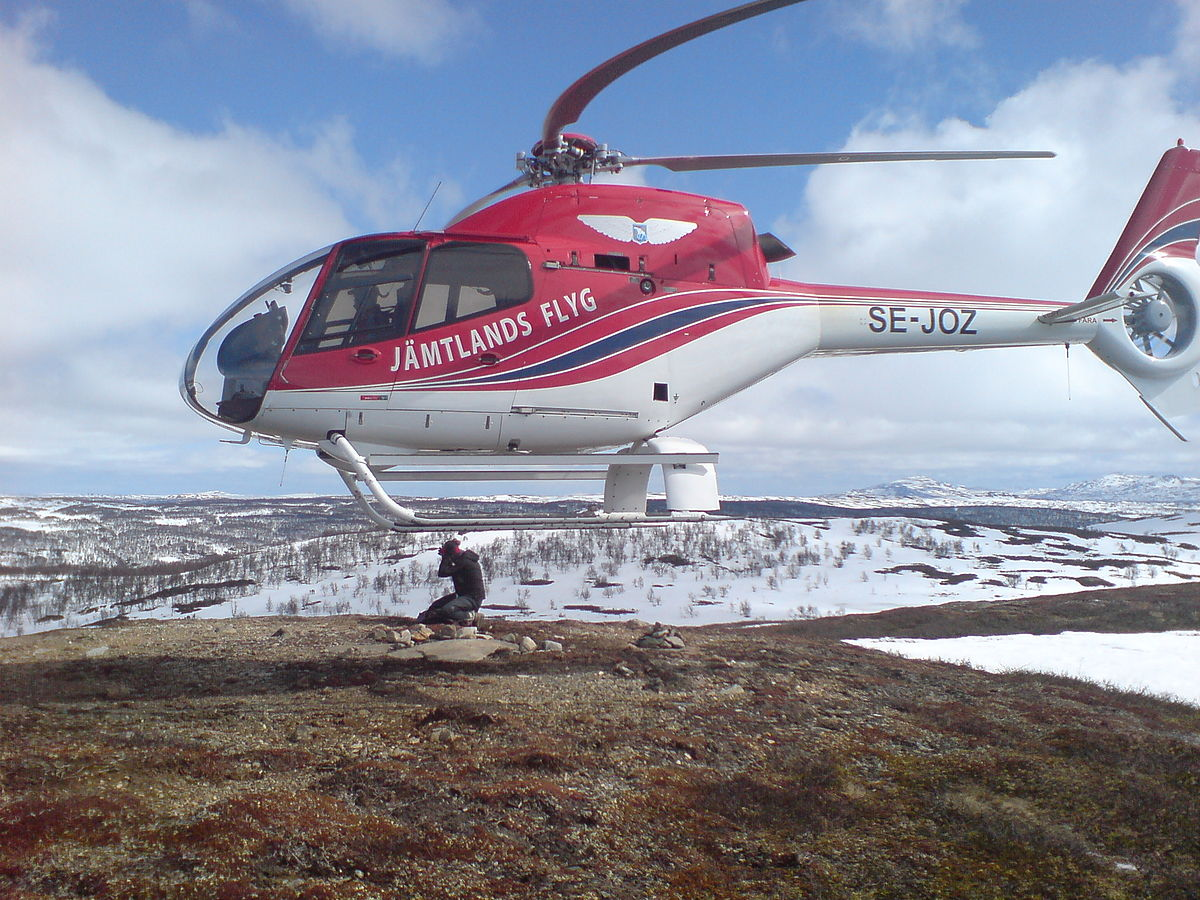
\includegraphics[width=0.49\linewidth]{img/rs1.jpeg}
		\includegraphics[width=0.49\linewidth]{img/rs2.jpg}
		\caption{\normf 卷帘相机拍摄飞机螺旋桨产生的畸变效应}
		\label{fig:卷帘快门拍摄飞机螺旋桨产生的畸变效应}
	\end{figure}
		
	
	\subsection{\normf{时空标定}}
	为了融合算法能够达到一个较好的精度,多个传感器之间的时空参数需要被准确地标定,也即多传感器时空标定。多传感器时空标定是一种技术,用于校准不同类型的传感器,如相机、雷达、激光、惯性测量单元等,以便它们可以在同一坐标系下同步地测量和记录时空数据。这种技术可以应用于自动驾驶、增强现实、机器人导航等领域,提高传感器的精度和鲁棒性。
	
	\section{\normf{文献调研}}
	为了对一个GS-camera/IMU系统进行标定,Mirzaei等人\cite{mirzaei2008kalman}实现了一个能够支持GS-Camera/IMU的VINS系统,进行了非常详细的参数可观性分析。该方法不需要靶标,通过引入IMU,标定相机/IMU参数,多次运行得到多相机参数。但是需要先验知识,即参数的初值,通过CAD量测获得,而且只支持GS相机的标定,不支持RS相机。
	为了实现离线的高精度时空标定,Furgale等人\cite{furgale2013unified}提出了一个基于连续时间优化框架的相机标定方法,也即Kalibr\footnote{\normf 该方法已在Github上开源:\url{https://github.com/ethz-asl/kalibr.git}},该方法需要靶标辅助,能够离线对时延进行标定,但是只支持GS相机的标定,不支持RS相机。
	
	为了支持RS相机的标定,槐等人\cite{huai2022continuous}基于Kalibr,扩展实现了RS相机的离线标定方法。在后面的工作中\cite{huai2022observability},他们实现了一个能够在线标定外参、时参、内参的VIO,不需要靶标辅助。该方法是基于扩展卡尔曼滤波实现的,实时性较强。
	
	上述的算法都是针对单个相机的标定方法。为了标定一套多相机系统,徐等人\cite{xu2022cammap}基于ORB-SLAM3实现的实时标定算法,其不需要靶标,不需要视场角重叠,支持多种相机类型(光学相机、深度相机、鱼眼相机、针孔相机),但是不支持RS相机。
	在工作\cite{furgale2012continuous}中,Furgale等人基于连续时间优化,实现了一套能够标定多个GS相机的离线标定方法。但是该方法不支持RS相机,同时需要棋盘格辅助。
	
	\section{\normf 方法设计}
	考虑到目前多相机标定方法的局限性,尤其是针对多个卷帘快门相机的标定,我们设计了一个基于连续时间的多卷帘快门相机的无靶标时空标定方法。主要的考量点有:
	\begin{enumerate}
	\item 如果设计的是一种无靶标的多相机标定,需要引入其他额外的尺度传感器(如IMU、LiDAR):
	\begin{enumerate}
	\item 单目相机是无深度(尺度)量测能力的,使用棋盘格引入了尺度信息(格子的真实长度);
	\item 如果没有棋盘格,不引入其他尺度传感器,多相机标定的结果中,外参位移是无尺度的;
	\item 用IMU辅助!IMU中的加速度计是有尺度的。而且IMU是万金油,几乎智能设备的装载;
	\item 没有靶标辅助,可以做到“现场标定”;
	\end{enumerate}
	
	\item 如果要标定多个RS相机,最好使用基于连续时间的估计方法:
	\begin{enumerate}
	\item 可以将RS效应非常精确地去除,非常有利于异步数据的融合;
	
	\item 能够非常方便的估计时延;
	
	\item 保证了运动的连续性的假设;
	\end{enumerate}
	\end{enumerate}
	
	\begin{figure}[h]
		\centering
		\includegraphics[width=\linewidth]{img/system.pdf}
		\caption{\normf 方法流程}
		\label{fig:方法流程}
	\end{figure}
	我们设计的方法的主要步骤如图\ref{fig:方法流程}所示。具体来说,算法主要包含四个步骤:$(i)$ 初始化:使用基于连续时间的预积分初始化方法进行外参、样条、重力向量、尺度的初始化;
	$(ii)$ 数据关联:基于SfM得到的结构构建视觉特征关联;
	$(iii)$  批处理优化:构建一个包含先验因子、视觉重投影因子、IMU因子和相关待优化参数的因子图,进行批处理优化;
	$(iv)$ 细化(精化):基于一定的策略进行参数优化控制,保证收敛的速度和结果的精度。
	
	这里主要介绍初始化模块。初始化方法是一个基于连续时间预积分的初始化策略,如图\ref{fig:基于连续时间预积分的初始化}所示。算法主要包含步骤:$(i)$ SO3样条拟合(使用IMU中的陀螺仪的输出);$(ii)$ SfM算法恢复各个相机的视觉结构(此时相机的尺度是未知的);$(iii)$ 手眼标定初始化外参姿态;$(iv)$ 预积分初始化其他参数(受VINS-Mono启发),注意到此时相机的尺度是可以确定的;$(v)$ 最后初始化位置样条.
	\begin{figure}[h]
		\centering
		\includegraphics[width=\linewidth]{img/ct_preintegration.pdf}
		\caption{\normf 基于连续时间预积分的初始化}
		\label{fig:基于连续时间预积分的初始化}
	\end{figure}
	
	\section{\normf{实验验证}}
		\begin{figure}[h]
			\centering
			\includegraphics[width=\linewidth]{img/simu_opt_process.pdf}
			\caption{\normf 参数收敛过程}
			\label{fig:参数收敛过程}
		\end{figure}
	图\ref{fig:参数收敛过程}绘制了不同过程中时空参数的收敛性能。
	可以看出,预积分后外旋转和平移的精度分别可以达到厘米级和度级。
	在下面的$\mathbb{R}^3$ B样条初始化中,这些参数被细化到更好的状态。
	随后,进行四次批量优化,在全局最小二乘问题中再次细化所有参数,保证了高精度的校准结果。
	我们发现,外部状态在 $\mathbb{R}^3$ B 样条初始化过程的前几次迭代中表现出较大的波动。
	这是由于大量未初始化的$\mathbb{R}^3$控制点与其他参数一起被优化,使得问题的非线性更强。
	应该指出的是,由于时空参数通常被视为已知并在估计器中固定,因此采用所提出的基于连续时间的预积分初始化方法进行初始化的辅助 INS 可以获得更好的性能。
	
	\begin{figure}[h]
		\centering
		\includegraphics[width=\linewidth]{img/maps.png}
		\caption{\normf 稀疏视觉地标地图}
		\label{fig:稀疏视觉地标地图}
	\end{figure}
	
	为了进一步评估初始化性能和校准结果,初始化和四批优化后的稀疏视觉地标图被构建,如图 \ref{fig:稀疏视觉地标地图} 所示。
	经过四次批量优化,两张地图的锯齿效应被消除,几何结构更加清晰,与真实场景更加吻合。
	还基于合并地图和估计的重力矢量构建了如图\ref{fig:稀疏视觉地标地图}右侧所示的彩色地图,以评估时空参数的校准一致性。
	颜色变化代表重力方向上的距离。
	显然,相机维护的地标地图中结构的高程变化与 IMU 维护的重力方向一致,这证明了我们方法的一致性。
	这得益于引入的虚拟中央 IMU,其 B 样条轨迹将所有时空参数连接到一个统一的优化问题中。

	\section{\normf{结论与展望}}
	在本文中,我们提出了一种基于连续时间估计的多异构相机和 IMU 的时空校准方法,该方法不需要先验知识或校准基础设施,并且能够实现内在精化。
	特别是,开发了一种新颖的基于连续时间的预积分初始化方法来执行初始化。
	此外,通过引入虚拟中央IMU,所有参数可以在一致的估计器中联合优化,从而保证了校准的一致性。
	在模拟和现实环境中进行了大量的实验,以评估所提出方法的可行性和有效性。
	结果表明,所提出的方法能够进行精确的时空和本征校准,并且优于其他最先进的方法。
	在未来的工作中,我们将进一步提高所提出方法的计算效率并将其应用于实时应用中。
	此外,该系统还将涉及更多类型的摄像机,例如事件摄像机、红外摄像机等。
	
	\bibliographystyle{IEEEtran}
	\bibliography{reference}
	
	\section*{ACKNOWLEDGMENT}
	\begin{tcolorbox}[colback=white,colframe=white!70!black,title={\bfseries Author Information}]
	\par\noindent
		\parbox[t]{\linewidth}{
	 \noindent\parpic{\includegraphics[height=2in,width=1in,clip,keepaspectratio]{ShuolongChen_grey.jpg}}
	 \noindent{\bfseries Shuolong Chen}\emph{
	 received the B.S. degree in geodesy and geomatics engineering from Wuhan University, Wuhan China, in 2023.
	 He is currently a master candidate at the school of Geodesy and Geomatics, Wuhan University. His area of research currently focuses on integrated navigation systems and multi-sensor fusion.
	 Contact him via e-mail: shlchen@whu.edu.cn.
	 }}
	\end{tcolorbox}
		
		
\end{document}

